
\section{Appendix for MS2}

\begin{figure}[H]
    \centering
    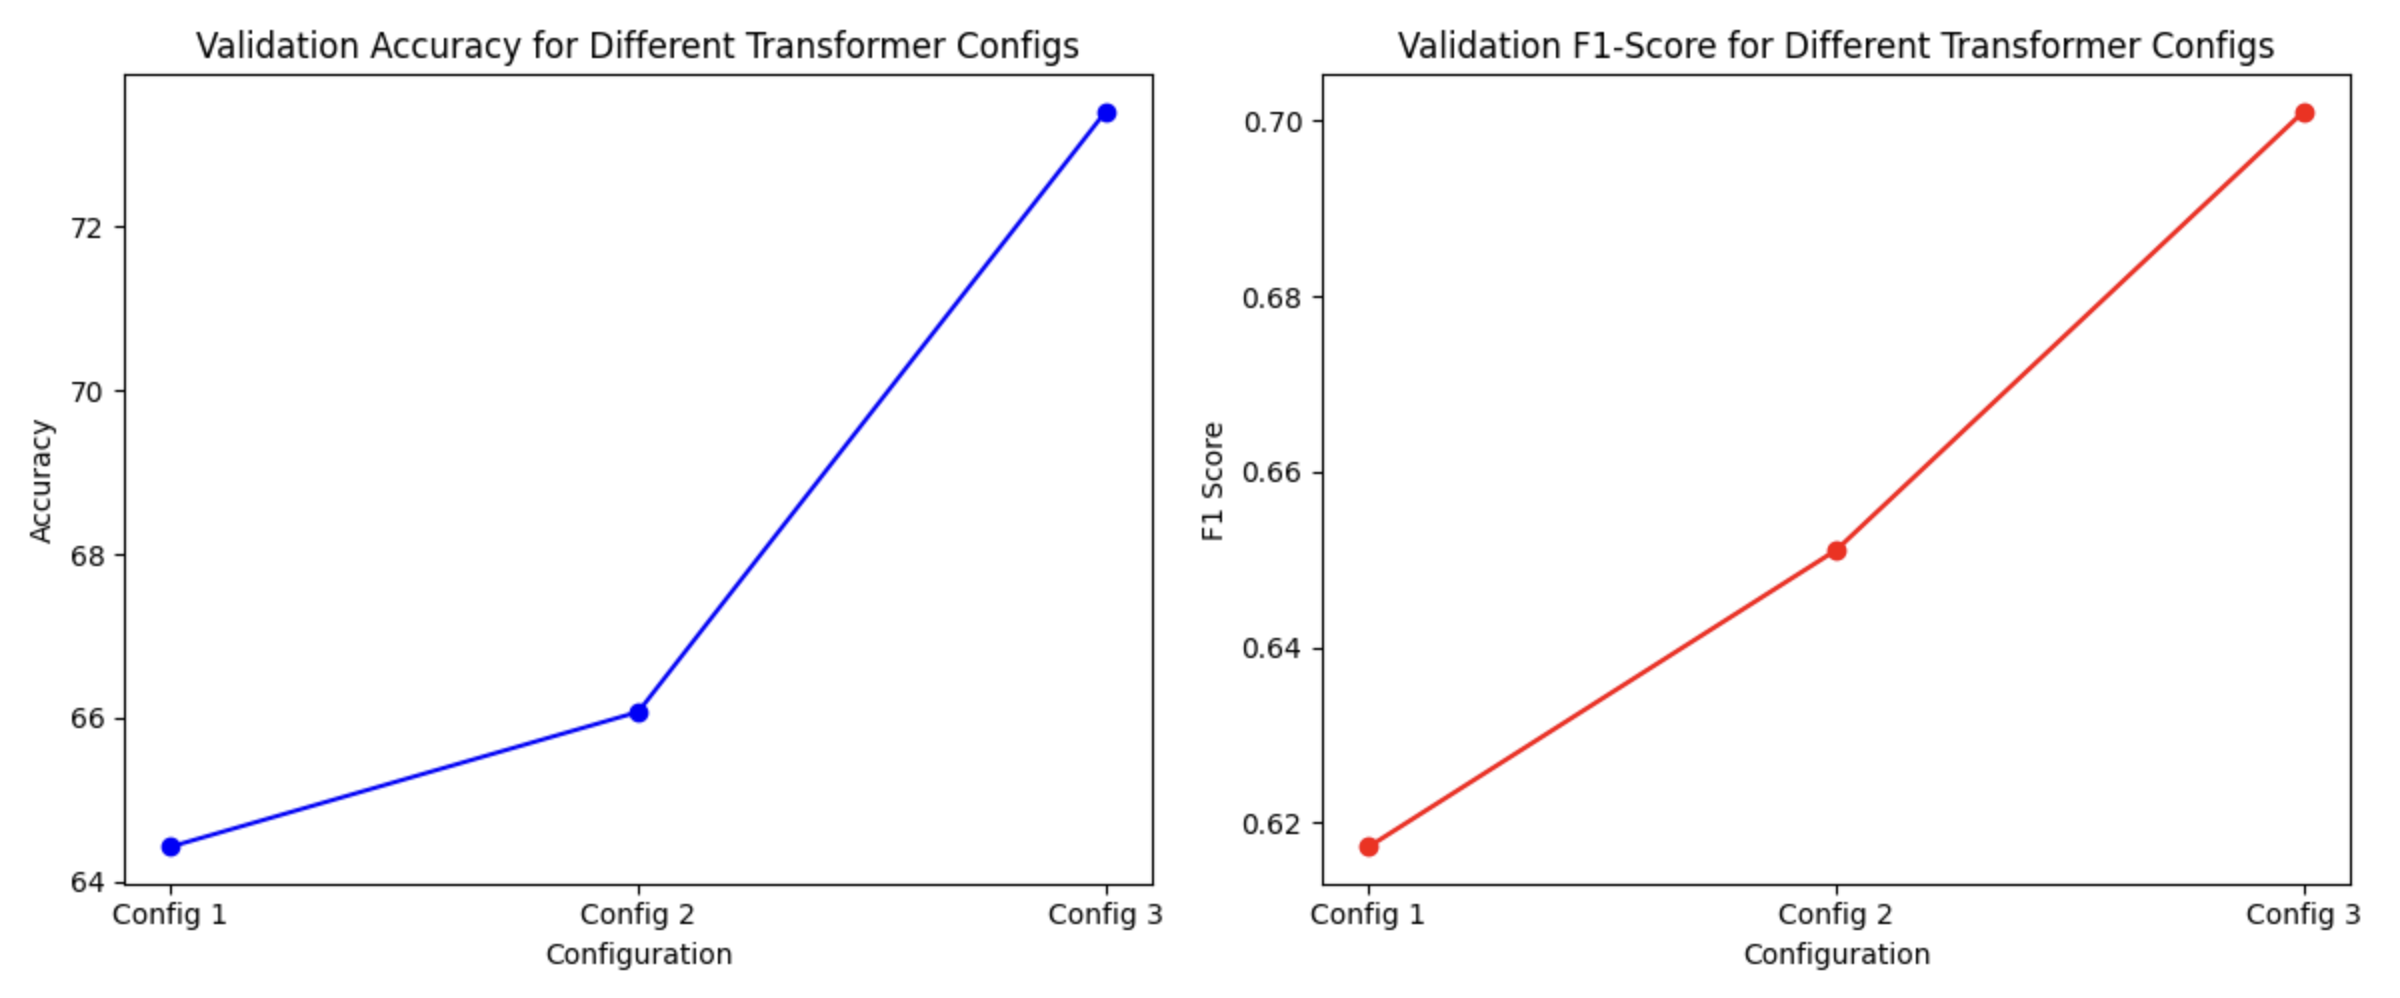
\includegraphics[width=0.6\linewidth]{images/transformer.png}
    \caption{Performance of the Transformer model across different datasets.}
    \label{fig:transformer}
\end{figure}

\begin{figure}[H]
    \centering
    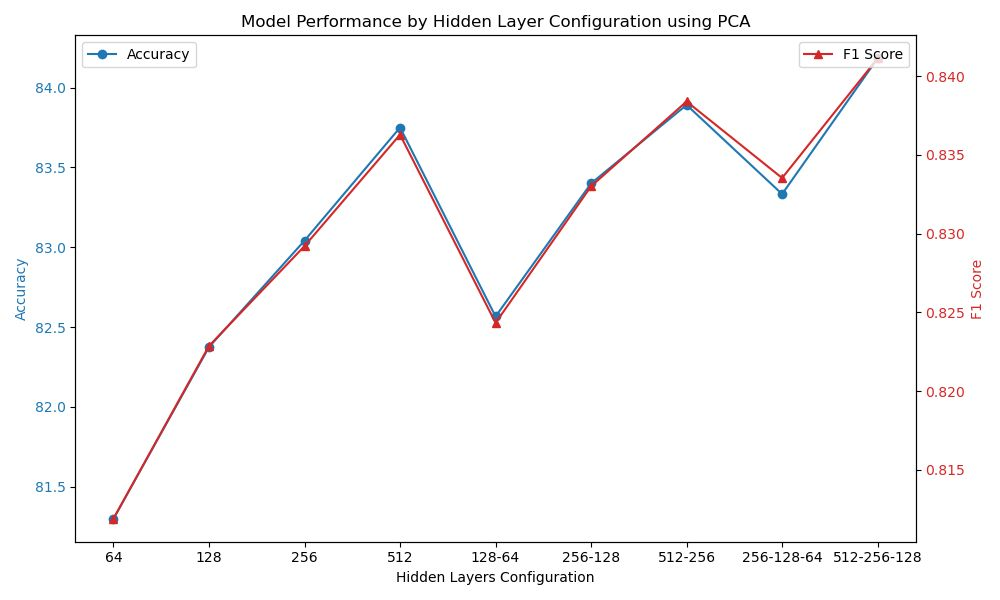
\includegraphics[width=0.6\linewidth]{images/model_performance_PCA.jpeg}
    \caption{Comparison of model performance with and without PCA feature reduction.}
    \label{fig:model_performance_PCA}
\end{figure}

\begin{figure}[H]
    \centering
    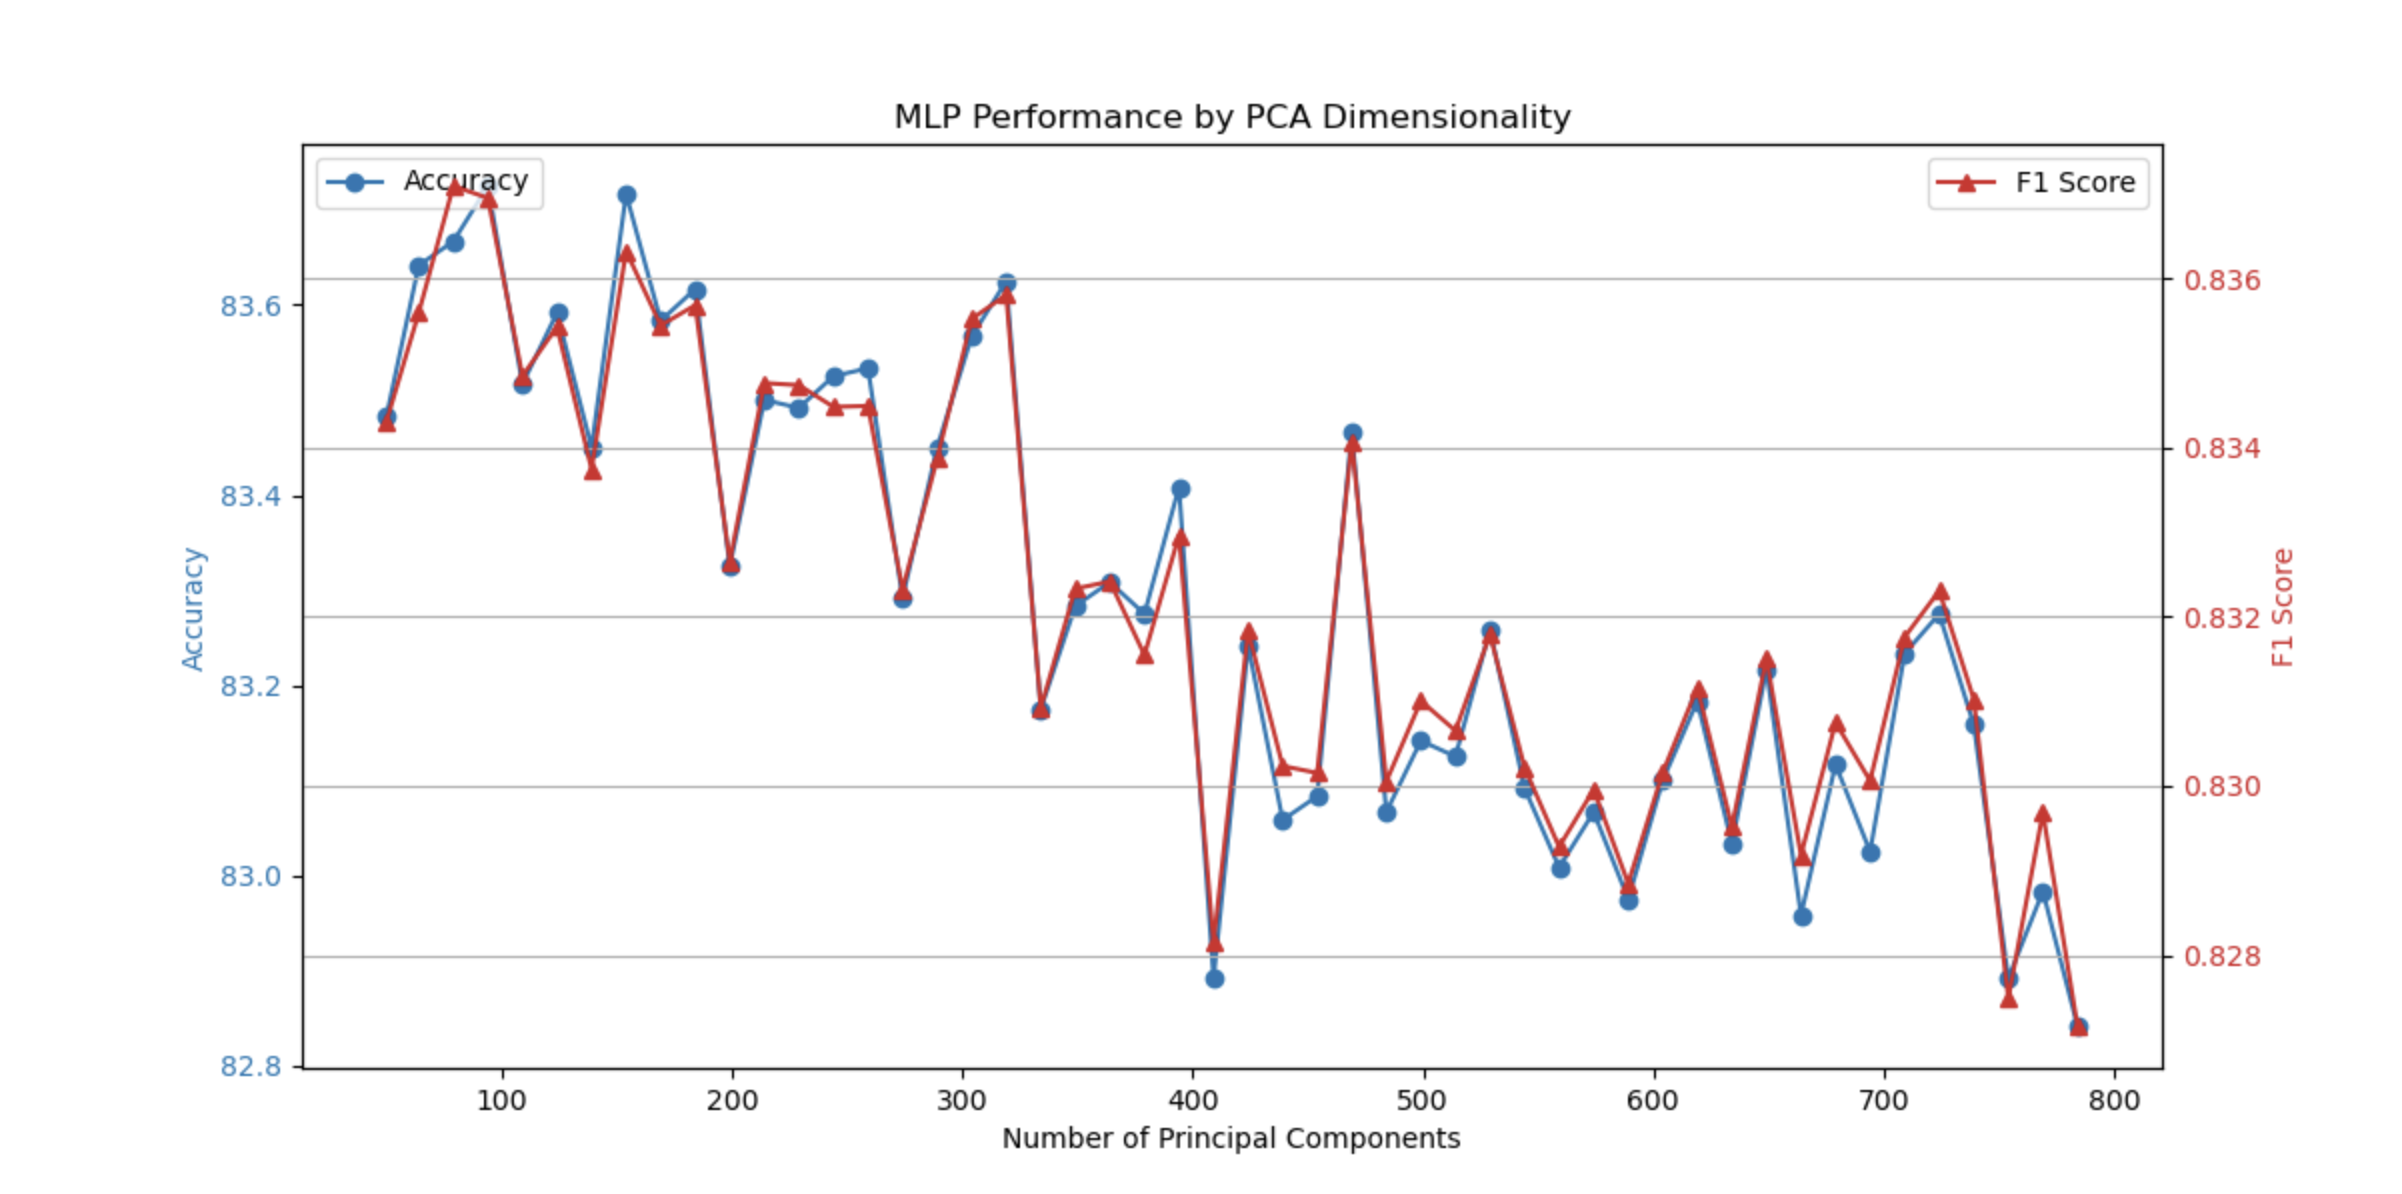
\includegraphics[width=0.6\linewidth]{images/pca.png}
    \caption{Comparison of model performance with different pca dimensions ranging from 50 to 784}
    \label{fig:model_performance_PCA2}
\end{figure}
\begin{figure}[H]
    \centering
    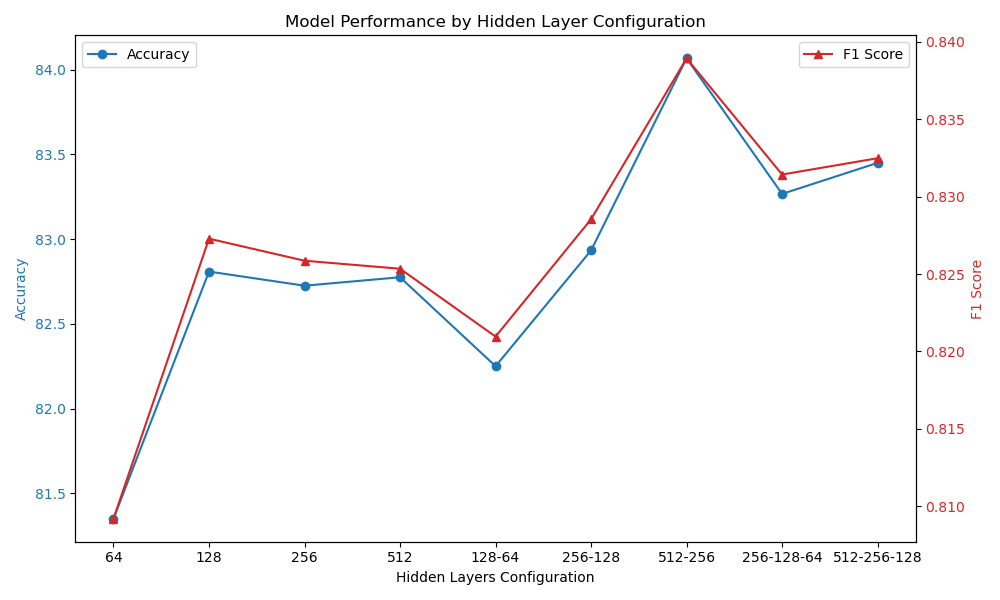
\includegraphics[width=0.6\linewidth]{images/model_performance.png}
    \caption{Overall performance metrics for the MLP model on the test set.}
    \label{fig:mlp_model_performance}
\end{figure}

\begin{table}[h!]
\centering
\begin{tabular}{>{\raggedright}p{4cm} >{\raggedleft}p{4cm} >{\raggedleft\arraybackslash}p{3cm}}
\toprule
\textbf{Layer (type)} & \textbf{Output Shape} & \textbf{Param \#} \\
\midrule
Conv2d              & [batch\_size, 128, 28, 28] & 1,280 \\
ReLU                 & [batch\_size, 128, 28, 28] & - \\
BatchNorm2d          & [batch\_size, 128, 28, 28] & 256 \\
Conv2d              & [batch\_size, 128, 28, 28] & 147,584 \\
ReLU                & [batch\_size, 128, 28, 28] & - \\
BatchNorm2d          & [batch\_size, 128, 28, 28] & 256 \\
MaxPool2d            & [batch\_size, 128, 14, 14] & - \\
Dropout              & [batch\_size, 128, 14, 14] & - \\
Conv2d               & [batch\_size, 256, 14, 14] & 295,168 \\
ReLU                & [batch\_size, 256, 14, 14] & - \\
BatchNorm2d         & [batch\_size, 256, 14, 14] & 512 \\
Conv2d              & [batch\_size, 256, 14, 14] & 590,080 \\
ReLU                & [batch\_size, 256, 14, 14] & - \\
BatchNorm2d         & [batch\_size, 256, 14, 14] & 512 \\
MaxPool2d           & [batch\_size, 256, 7, 7] & - \\
Dropout             & [batch\_size, 256, 7, 7] & - \\
Conv2d              & [batch\_size, 512, 7, 7] & 1,180,160 \\
ReLU                & [batch\_size, 512, 7, 7] & - \\
BatchNorm2d         & [batch\_size, 512, 7, 7] & 1,024 \\
MaxPool2d           & [batch\_size, 512, 3, 3] & - \\
Dropout             & [batch\_size, 512, 3, 3] & - \\
Flatten             & [batch\_size, 4608] & 0 \\
Linear              & [batch\_size, 512] & 2,359,808 \\
ReLU                & [batch\_size, 512] & - \\
BatchNorm1d         & [batch\_size, 512] & 1,024 \\
Dropout             & [batch\_size, 512] & - \\
Linear              & [batch\_size, 256] & 131,328 \\
ReLU                & [batch\_size, 256] & - \\
BatchNorm1d         & [batch\_size, 256] & 512 \\
Dropout            & [batch\_size, 256] & - \\
Linear              & [batch\_size, 10] & 2,570 \\
\bottomrule
\end{tabular}
\caption{CNN Architecture Summary}
\label{tab:model-summary}
\end{table}

\section*{Parameter Counts}

\begin{itemize}
    \item \textbf{Total parameters:} 4,712,074
    \item \textbf{Trainable parameters:} 4,712,074
    \item \textbf{Non-trainable parameters:} 0
\end{itemize}
